\begin{enumerate}
    \item A partir del circuito de la figura \ref{fig:topologias-basicas} determinar las conexiones necesarias para obtener un:
        \begin{itemize}
            \item Amplificador inversor.
            \item Amplificador no inversor.
            \item Amplificador restador.
            \item Convertidor de tensión a corriente.
            \item Circuito integrador no inversor (Integrador de Boo).
        \end{itemize}

    \item Escoger los valores de las resistencias para obtener un restador de ganancia 2, un inversor de ganancia -2, un amplificador no inversor. Para el integrador utilice un condensador de poliéster de $10nF$.

\end{enumerate}

\begin{figure}[ht]
    \centering
    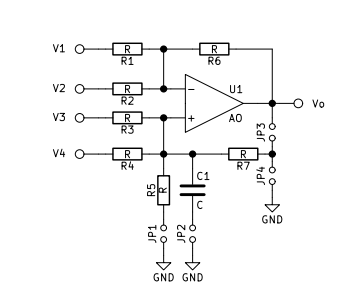
\includegraphics[width=0.5\textwidth]{topologias-basicas.png}
    \caption{Topologías básicas}
    \label{fig:topologias-basicas}
\end{figure}

\subsubsection{Amplificador inversor}

Para construir un inversor a partir de la topología base, se realizarán las siguientes conexiones:

\begin{itemize}
    \item a fuente: $v_1$
    \item a tierra: $JP1$
    \item abierto: $\volt{2}$, $\volt{3}$, $\volt{4}$, $\jumper{2}$, $\jumper{3}$, $\jumper{4}$
\end{itemize}

Para que la ganancia sea $-2$, debemos usar la formula \ref{eq:mt-ganancia-amp-inversor}, y seleccionar una resistencia $R_1$ cualquiera, en este caso se escoge $R_1 = 10k\Omega$, por lo que:

\begin{align*}
    r_6 &= -A \cdot R_1 \\
    r_6 &= - (-2) \cdot 10k\Omega \\
    r_6 &= 20k\Omega
\end{align*}

En la ilustración \ref{ilus:sim-amp-inversor} podemos observar la simulación del amplificador no inversor, y en la ilustración \ref{ilus:sim-amp-inversor-ganancia} podemos ver que la ganancia es -2, que corresponde con el valor teórico.

\begin{ilustracion}[ht]
    \centering
    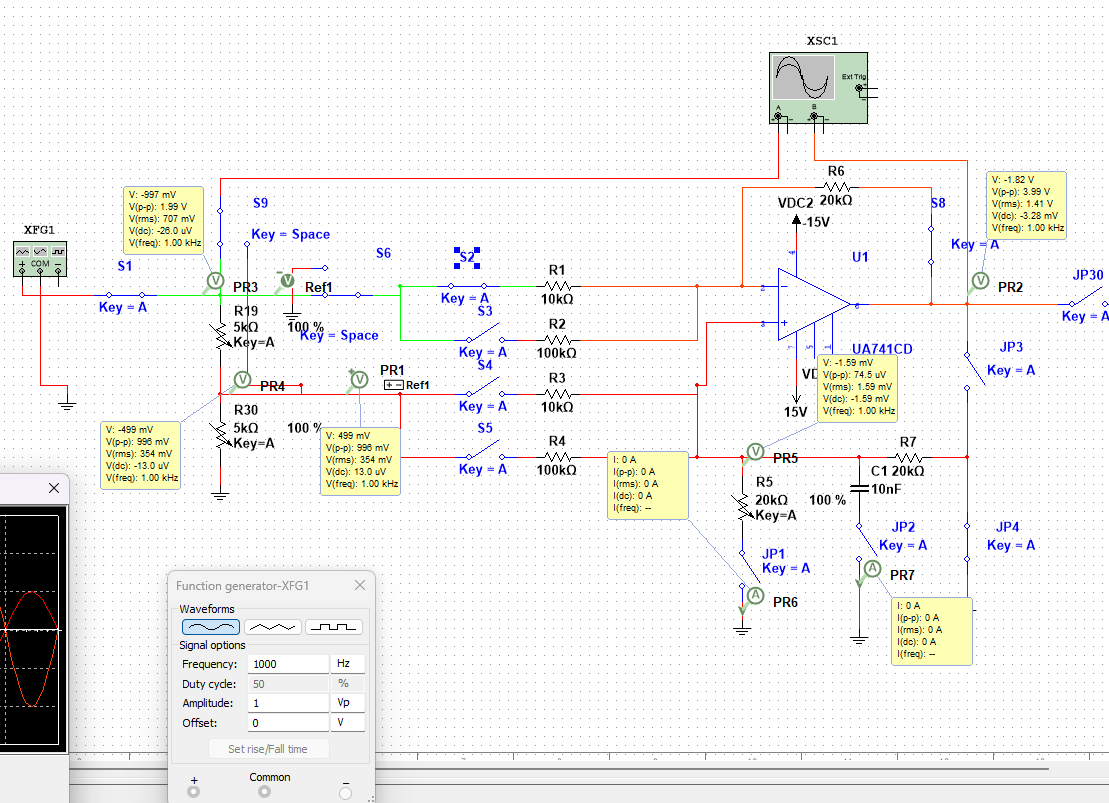
\includegraphics[width=0.8\textwidth]{simulaciones/amp-inversor.png}
    \caption{Simulación amplificador inversor}
    \label{ilus:sim-amp-inversor}
\end{ilustracion}

\begin{ilustracion}[ht]
    \centering
    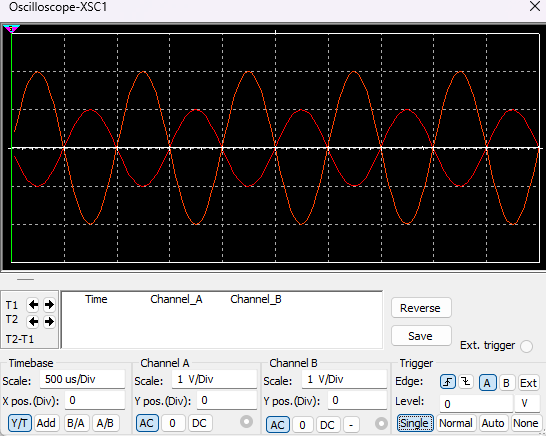
\includegraphics[width=0.8\textwidth]{simulaciones/amp-inversor-ganancia.png}
    \caption{Simulación ganancia amplificador inversor}
    \label{ilus:sim-amp-inversor-ganancia}
\end{ilustracion}

\subsubsection{Amplificador restador}

Para construir un restador a partir de la topología base, se realizarán las siguientes conexiones:

\begin{itemize}
    \item a fuente: $\volt{1}$ y $\volt{3}$
    \item a tierra: $\jumper{4}$
    \item abierto: $\volt{2}$, $\volt{4}$, $\jumper{1}$, $\jumper{2}$, $\jumper{3}$
\end{itemize}

\newcommand{\res}[1]{$r_{#1}$}

Utilizando las mismas resistencias \res{1} y \res{2} que en inversor  y la condición de que \res{1} = \res{3} y \res{6} = \res{7}, obtenemos:  

\begin{align*}
    R_3 &= R_1 = 10k\Omega \\
    R_7 &= R_6 = 20k\Omega \\
\end{align*}

Ahora podemos utilizar la formula simplificada de ganancia del restador (\ref{eq:mt-ganancia-restador}):


\begin{align*}
    A &= \frac{v_0}{v_2 - v_1} \\
    A & = \frac{R_6}{R_1} = 2 \\
    A &= \frac{20k\Omega}{10k\Omega} = 2
\end{align*}

En la ilustración \ref{ilus:sim-amp-restador} podemos observar la simulación del amplificador no inversor, y en la ilustración \ref{ilus:sim-amp-restador-ganancia} podemos ver que la ganancia es 2, que corresponde con el valor teórico. Aunque pareciera que las señales de entrada y salida están desfasadas, eso es debido a que $V_2 < V_1$

\begin{ilustracion}[ht]
    \centering
    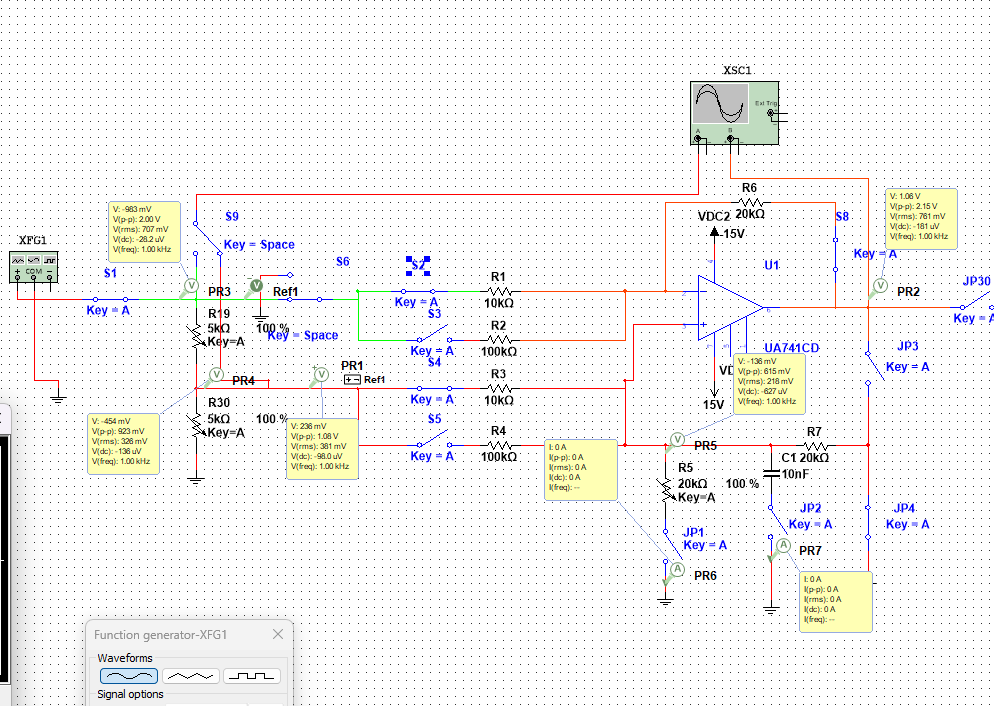
\includegraphics[width=0.8\textwidth]{simulaciones/amp-restador.png}
    \caption{Simulación amplificador restador}
    \label{ilus:sim-amp-restador}
\end{ilustracion}

\begin{ilustracion}[ht]
    \centering
    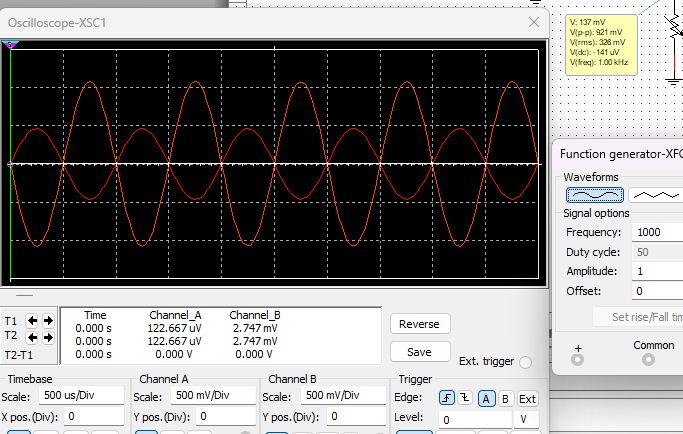
\includegraphics[width=0.8\textwidth]{simulaciones/amp-restador-ganancia.png}
    \caption{Simulación ganancia amplificador restador}
    \label{ilus:sim-amp-restador-ganancia}
\end{ilustracion}


\FloatBarrier
\subsubsection{Amplificador no inversor}

Para construir un no inversor a partir de la topología base, se realizarán las siguientes conexiones:

\begin{itemize}
    \item a fuente: $\volt{3}$
    \item a tierra: $\volt{1}$
    \item abierto: $\volt{2}$, $\volt{4}$, $\jumper{1}$, $\jumper{2}$, $\jumper{3}$, $\jumper{4}$
\end{itemize}

Siguiendo la formula de ganancia del no inversor (\ref{eq:mt-ganancia-amp-no-inversor}), y utilizando las resistencias $r_3$ y $r_6$ utilizadas anteriormente, se obtiene:

\begin{align*}
    A = 1 + \frac{r_3}{r_6} \\
    A = 1 + \frac{20k\Omega}{10k\Omega} = 3
\end{align*}

En la ilustración \ref{ilus:sim-amp-no-inversor} podemos observar la simulación del amplificador no inversor, y en la ilustración \ref{ilus:sim-amp-no-inversor-ganancia} podemos ver que la ganancia es 3, que corresponde con el valor teórico.

\begin{ilustracion}[ht]
    \centering
    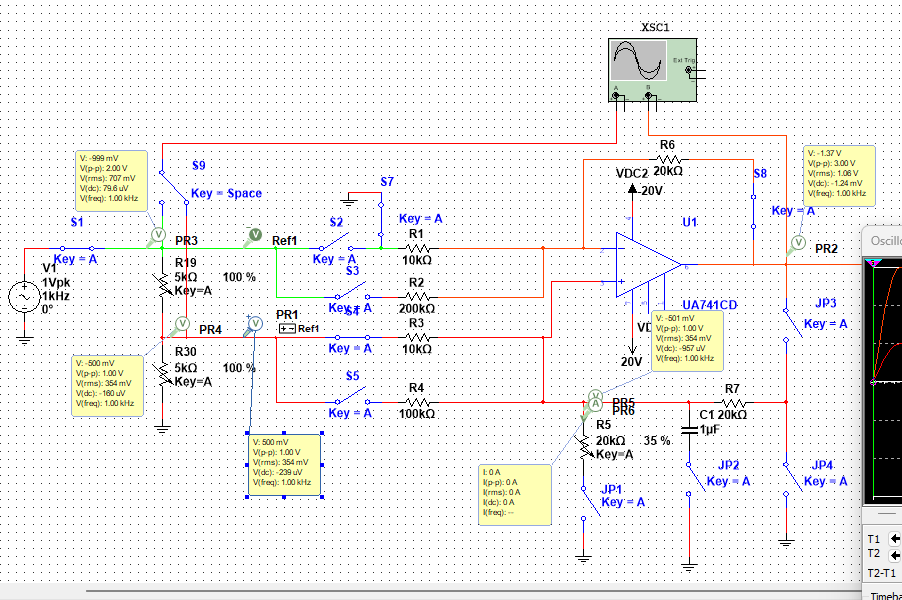
\includegraphics[width=0.8\textwidth]{simulaciones/conexion-no-inversor.png}
    \caption{Simulación amplificador no inversor}
    \label{ilus:sim-amp-no-inversor}
\end{ilustracion}

\begin{ilustracion}[ht]
    \centering
    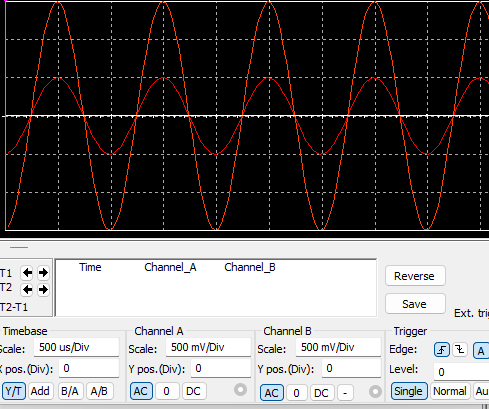
\includegraphics[width=0.8\textwidth]{simulaciones/ganancia-no-inversor.png}
    \caption{Simulación ganancia amplificador no inversor}
    \label{ilus:sim-amp-no-inversor-ganancia}
\end{ilustracion}

\FloatBarrier
\subsubsection{Fuente de corriente}

Para construir un convertidor de tensión a corriente a partir de la topología base, se realizarán las siguientes conexiones:

\begin{itemize}
    \item a fuente: $\volt{4}$
    \item a tierra: $\volt{2}$, $\jumper{1}$
    \item abierto: $\volt{1}$, $\volt{3}$, $\jumper{2}$, $\jumper{4}$
    \item cerrado: $\jumper{3}$
\end{itemize}

Para esta conexión se utilizarán las mismas resistencias \res{6} = \res{7} que con las conexiones anteriores, sin embargo, para aumentar la estabilidad de la salida, es necesario que $R_1 \gg R_7$, por ello, para las entradas $\volt{2}$ y $\volt{4}$ se escogeran las resistencias:

\begin{align*}
    R_2 &= R_4 = 100k\Omega \\
\end{align*}

Ahora, utilizando la formula (\ref{eq:mt-io-fuente-corriente}) y asumiendo un voltaje de entrada $v_i = 1Vp$ obtenemos:

\begin{align*}
    i_o &= \frac{v_i}{R_1}  \\
    i_o &= \frac{1V}{100k\Omega}  \\
    i_o & = 10\mu A
\end{align*}

En la ilustración \ref{ilus:sim-fuente-corriente} podemos observar el circuito de la fuente de corriente. Y en las siguientes ilustracións podemos observar que para distintos valores de resistencias (20k, 16k, 5k y 1k) obtuvimos valores cercanos a $10\mu A$, que fue el valor esperado.

\begin{ilustracion}[ht]
    \centering
    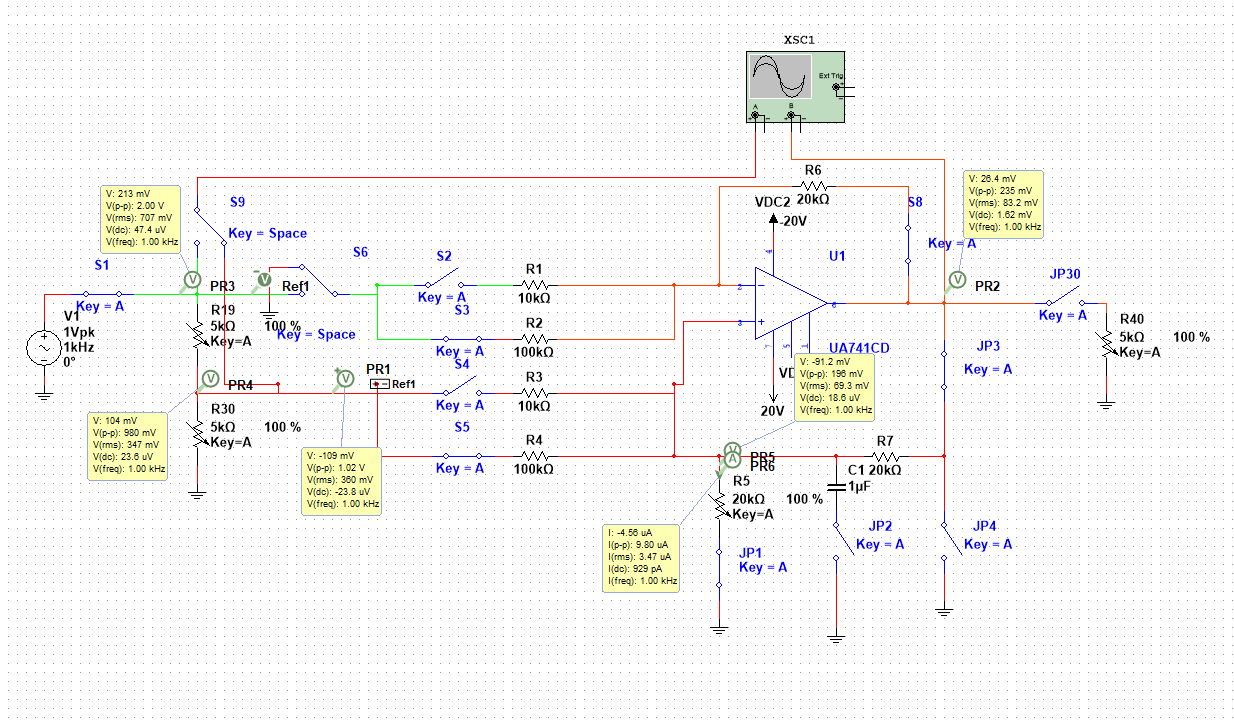
\includegraphics[width=0.8\textwidth]{simulaciones/fuente-corriente-rango-amplio.png}
    \caption{Simulación circuito fuente de corriente}
    \label{ilus:sim-fuente-corriente}
\end{ilustracion}
\begin{ilustracion}[ht]
    \centering
    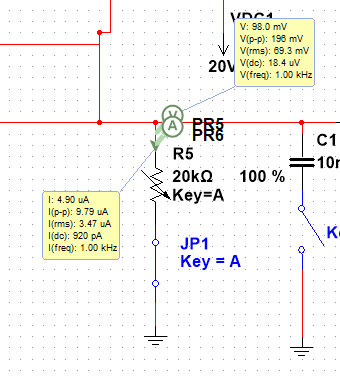
\includegraphics[width=0.3\textwidth]{simulaciones/fuente-corriente-mejor-20k.png}
    \caption{I y V de la fuente de corriente con R=20k}
    \label{ilus:sim-fuente-corriente-20k}
\end{ilustracion}
\begin{ilustracion}[ht]
    \centering
    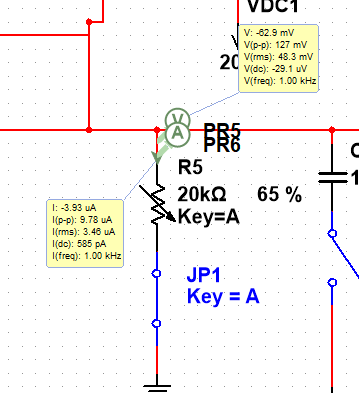
\includegraphics[width=0.3\textwidth]{simulaciones/fuente-corriente-mejor-13k.png}
    \caption{I y V de la fuente de corriente con R=20k}
    \label{ilus:sim-fuente-corriente-13k}
\end{ilustracion}
\begin{ilustracion}[ht]
    \centering
    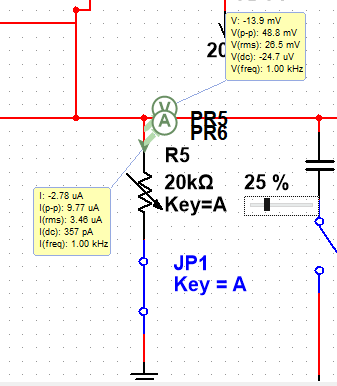
\includegraphics[width=0.3\textwidth]{simulaciones/fuente-corriente-mejor-5k.png}
    \caption{I y V de la fuente de corriente con R=5k}
    \label{ilus:sim-fuente-corriente-5k}
\end{ilustracion}
\begin{ilustracion}[ht]
    \centering
    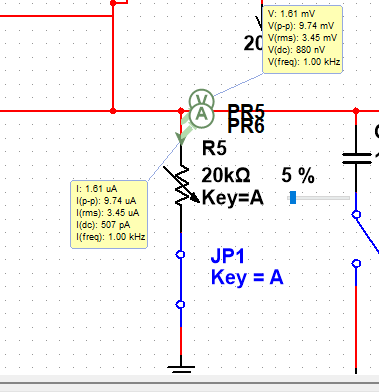
\includegraphics[width=0.3\textwidth]{simulaciones/fuente-corriente-mejor-1k.png}
    \caption{I y V de la fuente de corriente con R=1k}
    \label{ilus:sim-fuente-corriente-1k}
\end{ilustracion}


\FloatBarrier
\subsubsection{Integrador no inversor}

Para construir el integrador no inversor, simplemente sustituimos la carga $R_5$ por una capacitancia $C_1 = 10nF$ en la fuente de voltaje, las conexiones serán las siguientes:

\begin{itemize}
    \item a fuente: $\volt{4}$
    \item a tierra: $\volt{2}$, $\jumper{2}$
    \item abierto: $\volt{1}$, $\volt{3}$, $\jumper{1}$, $\jumper{4}$
    \item cerrado: $\jumper{3}$
\end{itemize}

Este circuito debe integrar la señal de entrada. Si se la entrada es una señal cuadrada, la salida debe ser una señal triangular.

En la ilustración \ref{ilus:sim-integrador} podemos apreciar la conexión del circuito integrador.

En las siguientes ilustracións podemos observar la como el circuito integra la señal de entrada, en este caso una señal cuadrada se transforma en una rampa. Las zonas donde la señal se curva es poque se encuentra en la zona de saturación.

\begin{ilustracion}[ht]
    \centering
    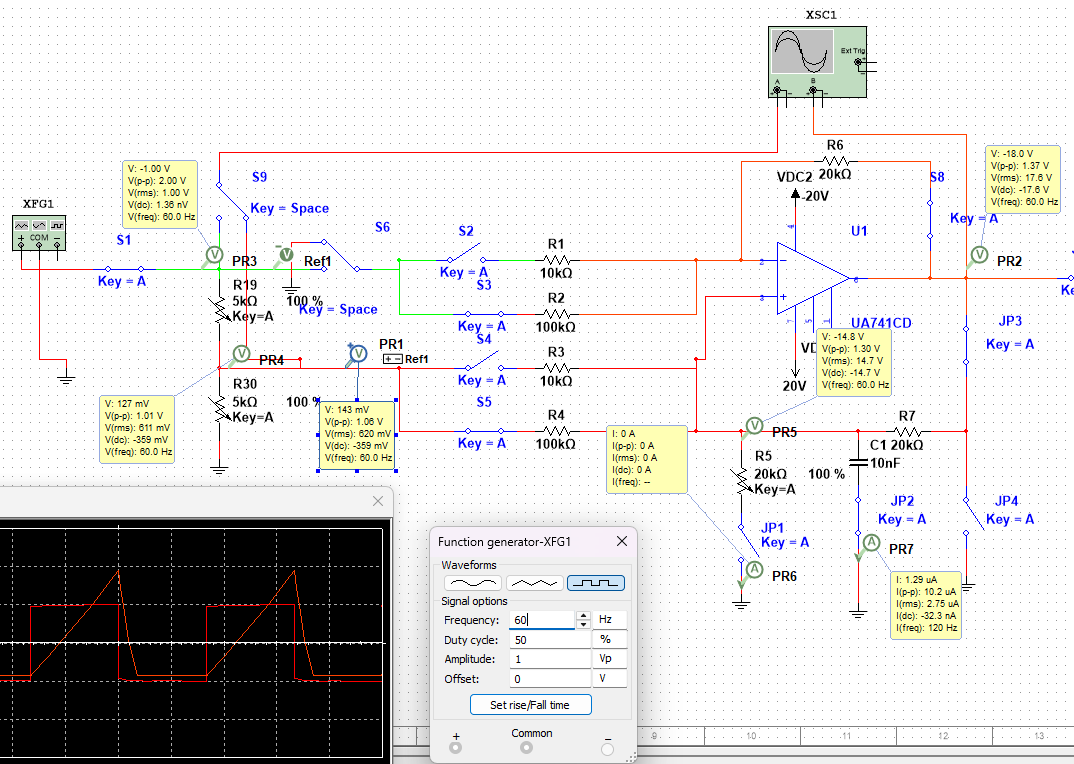
\includegraphics[width=0.6\textwidth]{simulaciones/integrador.png}
    \caption{Simulación circuito integrador Deboo}
    \label{ilus:sim-integrador}
\end{ilustracion}

\begin{ilustracion}[ht]
    \centering
    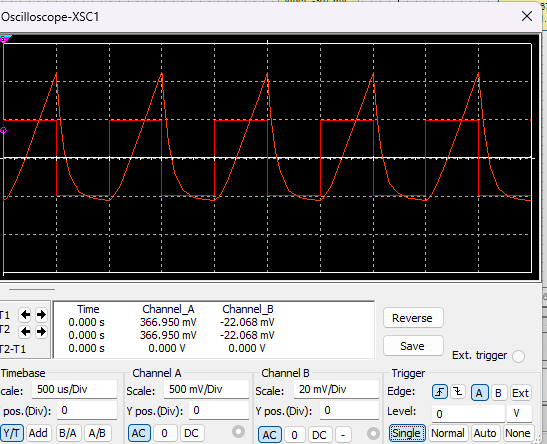
\includegraphics[width=0.3\textwidth]{simulaciones/integrador-transferencia-1khz.png}
    \caption{función de transferencia circuito integrador a 1kHz}
    \label{ilus:sim-integrador-1k}
\end{ilustracion}

\begin{ilustracion}[ht]
    \centering
    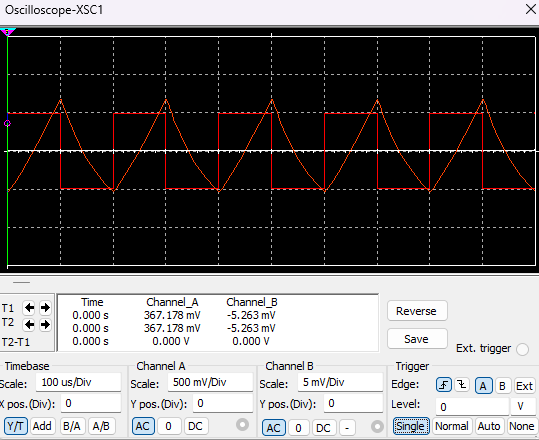
\includegraphics[width=0.3\textwidth]{simulaciones/integrador-transferencia-5kh.png}
    \caption{función de transferencia circuito integrador a 5kHz}
    \label{ilus:sim-integrador-5k}
\end{ilustracion}

\begin{ilustracion}[ht]
    \centering
    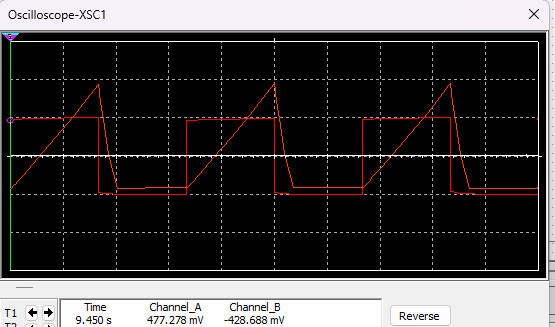
\includegraphics[width=0.3\textwidth]{simulaciones/integrador-transferencia-60hz.png}
    \caption{función de transferencia circuito integrador a 60Hz}
    \label{ilus:sim-integrador-60}
\end{ilustracion}